\subsection{Multidimensional arrays}

Internally, a multidimensional array is essentially the same thing as a linear array.

Since the computer memory is linear, it is an one-dimensional array.
For convenience, this multi-dimensional array can be easily represented as one-dimensional.

For example, this is how the elements of the 3x4 array are placed in one-dimensional array of 12 cells:

% TODO FIXME not clear. First, horizontal would be better. Second, why two columns?
% I'd first show 3x4 with numbered elements (e.g. 32-bit ints) in colored lines,
% then linear with the same numbered elements (and colored blocks)
% then linear with addresses (offsets) - assuming let say 32-bit ints.
\begin{table}[H]
\centering
\begin{tabular}{ | l | l | }
\hline
Offset in memory & array element \\
\hline
0 & [0][0] \\
\hline
1 & [0][1] \\
\hline
2 & [0][2] \\
\hline
3 & [0][3] \\
\hline
4 & [1][0] \\
\hline
5 & [1][1] \\
\hline
6 & [1][2] \\
\hline
7 & [1][3] \\
\hline
8 & [2][0] \\
\hline
9 & [2][1] \\
\hline
10 & [2][2] \\
\hline
11 & [2][3] \\
\hline
\end{tabular}
\caption{Two-dimensional array represented in memory as one-dimensional}
\end{table}

Here is how each cell of 3*4 array are placed in memory:

% TODO coordinates. TikZ?
\begin{table}[H]
\centering
\begin{tabular}{ | l | l | l | l | }
\hline                        
0 & 1 & 2 & 3 \\
\hline  
4 & 5 & 6 & 7 \\
\hline  
8 & 9 & 10 & 11 \\
\hline  
\end{tabular}
\caption{Memory addresses of each cell of two-dimensional array}
\end{table}

\myindex{row-major order}

So, in order to calculate the address of the element we need, we first multiply the first index by
4 (array width) and then add the second index.
That's called \IT{row-major order}, 
and this method of array and matrix representation is used in at least \CCpp and Python. 
The term \IT{row-major order} 
in plain English language means: \q{first, write the elements of the first row, then the second row \dots 
and finally the elements of the last row}.

\myindex{column-major order}
\myindex{Fortran}
Another method for representation is called \IT{column-major order} (the array indices are used in reverse order) 
and it is used at least in Fortran, MATLAB and R. 
\IT{column-major order} term in plain English language means: \q{first, write the elements of the first column, then the second column \dots
and finally the elements of the last column}.

Which method is better?

In general, in terms of performance and cache memory, 
the best scheme for data organization is the one,
in which the elements are accessed sequentially.

So if your function accesses data per row, \IT{row-major order} is better, and vice versa.

% subsections
\subsubsection{Two-dimensional array example}

We are going to work with an array of type \Tchar, which implies that each element requires only one 
byte in memory.

\myparagraph{Row filling example}
\myindex{\olly}

Let's fill the second row with these values 0..3:

\lstinputlisting[caption=Row filling example,style=customc]{patterns/13_arrays/5_multidimensional/two1_EN.c}

All three rows are marked with red. 
We see that second row now has values 0, 1, 2 and 3:

\begin{figure}[H]
\centering
\includegraphics[width=0.6\textwidth]{patterns/13_arrays/5_multidimensional/olly_2D_1.png}
\caption{\olly: array is filled}
\end{figure}

\myparagraph{Column filling example}
\myindex{\olly}

Let's fill the third column with values: 0..2:

\lstinputlisting[caption=Column filling example,style=customc]{patterns/13_arrays/5_multidimensional/two2_EN.c}

The three rows are also marked in red here. 

We see that in each row, at third position these values are written: 0, 1 and 2.

\begin{figure}[H]
\centering
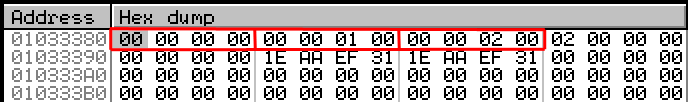
\includegraphics[width=0.6\textwidth]{patterns/13_arrays/5_multidimensional/olly_2D_2.png}
\caption{\olly: array is filled}
\end{figure}


\subsubsection{Access two-dimensional array as one-dimensional}

We can be easily assured that it's possible to access a two-dimensional array as one-dimensional array in at least two ways:

\lstinputlisting[style=customc]{patterns/13_arrays/5_multidimensional/2D_as_1D_EN.c}

Compile and run it: it shows correct values.

What MSVC 2013 did is fascinating, all three routines are just the same!

\lstinputlisting[caption=\Optimizing MSVC 2013 x64,style=customasmx86]{patterns/13_arrays/5_multidimensional/2D_as_1D_MSVC_2013_Ox_x64_EN.asm}

GCC also generates equivalent routines, but slightly different:

\lstinputlisting[caption=\Optimizing GCC 4.9 x64,style=customasmx86]{patterns/13_arrays/5_multidimensional/2D_as_1D_GCC49_x64_O3_EN.s}


\subsubsection{Three-dimensional array example}

It's the same for multidimensional arrays.

Now we are going to work with an array of type \Tint: each element requires 4 bytes in memory.

Let's see:

\lstinputlisting[caption=simple example,style=customc]{patterns/13_arrays/5_multidimensional/multi.c}

\myparagraph{x86}

We get (MSVC 2010):

\lstinputlisting[caption=MSVC 2010,style=customasmx86]{patterns/13_arrays/5_multidimensional/multi_msvc_EN.asm}

Nothing special. For index calculation, three input arguments are used 
in the formula $address=600 \cdot 4 \cdot x + 30 \cdot 4 \cdot y + 4z$, to represent the array as multidimensional.
Do not forget that the \Tint type is 32-bit (4 bytes),
so all coefficients must be multiplied by 4.

\lstinputlisting[caption=GCC 4.4.1,style=customasmx86]{patterns/13_arrays/5_multidimensional/multi_gcc_EN.asm}

The GCC compiler does it differently.

For one of the operations in the calculation ($30y$), GCC produces code without multiplication instructions.
This is how it done: 
$(y+y) \ll 4 - (y+y) = (2y) \ll 4 - 2y = 2 \cdot 16 \cdot y - 2y = 32y - 2y = 30y$. 
Thus, for the $30y$ calculation, only one addition operation,
one bitwise shift operation and one subtraction operation are used.
This works faster.

\myparagraph{ARM + \NonOptimizingXcodeIV (\ThumbMode)}

\lstinputlisting[caption=\NonOptimizingXcodeIV (\ThumbMode),style=customasmARM]{patterns/13_arrays/5_multidimensional/multi_Xcode_thumb_O0_EN.asm}

\NonOptimizing LLVM saves all variables in local stack, which is redundant.

The address of the array element is calculated by the formula we already saw.

\myparagraph{ARM + \OptimizingXcodeIV (\ThumbMode)}

\lstinputlisting[caption=\OptimizingXcodeIV (\ThumbMode),style=customasmARM]{patterns/13_arrays/5_multidimensional/multi_Xcode_thumb_O3_EN.asm}

The tricks for replacing multiplication by shift, addition and subtraction which we already saw
are also present here.

\myindex{ARM!\Instructions!RSB}
\myindex{ARM!\Instructions!SUB}
Here we also see a new instruction for us: \RSB (\IT{Reverse Subtract}).

It works just as \SUB, but it swaps its operands with each other before execution.
Why?
\myindex{ARM!Optional operators!LSL}
\SUB and \RSB  are instructions, to the second operand of which shift coefficient may be applied: (\INS{LSL\#4}). 

But this coefficient can be applied only to second operand.

That's fine for commutative operations like addition or multiplication 
(operands may be swapped there without changing the result).

But subtraction is a non-commutative operation, so \RSB exist for these cases.

\myparagraph{MIPS}

\myindex{MIPS!Global Pointer}
My example is tiny, so the GCC compiler decided to put the $a$ array into the 64KiB area 
addressable by the Global Pointer.

\lstinputlisting[caption=\Optimizing GCC 4.4.5 (IDA),style=customasmMIPS]{patterns/13_arrays/5_multidimensional/multi_MIPS_O3_IDA_EN.lst}



\subsubsection{More examples}

The computer screen is represented as a 2D array, but the video-buffer is a linear 1D array. 
We talk about it here: \myref{Mandelbrot_demo}.

Another example in this book is Minesweeper game: it's field is also two-dimensional array: \ref{minesweeper_winxp}.

